\documentclass[12pt,letterpaper]{article}
\usepackage[utf8]{inputenc}
\usepackage[spanish, es-tabla]{babel}
\usepackage[version=3]{mhchem}
\usepackage[journal=jacs]{chemstyle}
\usepackage{amsmath}
\usepackage{amsfonts}
\usepackage{amssymb}
\usepackage{makeidx}
\usepackage{xcolor}
\usepackage[stable]{footmisc}
\usepackage[section]{placeins}
%Paquetes necesarios para tablas
\usepackage{longtable}
\usepackage{array}
\usepackage{xtab}
\usepackage{multirow}
\usepackage{colortab}
%Paquete para el manejo de las unidades
\usepackage{siunitx}
\sisetup{mode=text, output-decimal-marker = {,}, per-mode = symbol, qualifier-mode = phrase, qualifier-phrase = { de }, list-units = brackets, range-units = brackets, range-phrase = --}
\DeclareSIUnit[number-unit-product = \;] \atmosphere{atm}
\DeclareSIUnit[number-unit-product = \;] \pound{lb}
\DeclareSIUnit[number-unit-product = \;] \inch{"}
\DeclareSIUnit[number-unit-product = \;] \foot{ft}
\DeclareSIUnit[number-unit-product = \;] \yard{yd}
\DeclareSIUnit[number-unit-product = \;] \mile{mi}
\DeclareSIUnit[number-unit-product = \;] \pint{pt}
\DeclareSIUnit[number-unit-product = \;] \quart{qt}
\DeclareSIUnit[number-unit-product = \;] \flounce{fl-oz}
\DeclareSIUnit[number-unit-product = \;] \ounce{oz}
\DeclareSIUnit[number-unit-product = \;] \degreeFahrenheit{\SIUnitSymbolDegree F}
\DeclareSIUnit[number-unit-product = \;] \degreeRankine{\SIUnitSymbolDegree R}
\DeclareSIUnit[number-unit-product = \;] \usgallon{galón}
\DeclareSIUnit[number-unit-product = \;] \uma{uma}
\DeclareSIUnit[number-unit-product = \;] \ppm{ppm}
\DeclareSIUnit[number-unit-product = \;] \eqg{eq-g}
\DeclareSIUnit[number-unit-product = \;] \normal{\eqg\per\liter\of{solución}}
\DeclareSIUnit[number-unit-product = \;] \molal{\mole\per\kilo\gram\of{solvente}}
\usepackage{cancel}
%Paquetes necesarios para imágenes, pies de página, etc.
\usepackage{graphicx}
\usepackage{lmodern}
\usepackage{fancyhdr}
\usepackage[left=4cm,right=2cm,top=3cm,bottom=3cm]{geometry}

%Instrucción para evitar la indentación
%\setlength\parindent{0pt}
%Paquete para incluir la bibliografía
\usepackage[backend=bibtex,style=chem-acs,biblabel=dot]{biblatex}
\addbibresource{references.bib}

%Formato del título de las secciones

\usepackage{titlesec}
\usepackage{enumitem}
\titleformat*{\section}{\bfseries\large}
\titleformat*{\subsection}{\bfseries\normalsize}

%Creación del ambiente anexos
\usepackage{float}
\floatstyle{plaintop}
\newfloat{anexo}{thp}{anx}
\floatname{anexo}{Anexo}
\restylefloat{anexo}
\restylefloat{figure}

%Modificación del formato de los captions
\usepackage[margin=10pt,labelfont=bf]{caption}

%Paquete para incluir comentarios
\usepackage{todonotes}

%Paquete para incluir hipervínculos
\usepackage[colorlinks=true,
            linkcolor = blue,
            urlcolor  = blue,
            citecolor = black,
            anchorcolor = blue]{hyperref}

%%%%%%%%%%%%%%%%%%%%%%
%Inicio del documento%
%%%%%%%%%%%%%%%%%%%%%%

\begin{document}
\renewcommand{\labelitemi}{$\checkmark$}

\renewcommand{\CancelColor}{\color{red}}

\newcolumntype{L}[1]{>{\raggedright\let\newline\\\arraybackslash}m{#1}}

\newcolumntype{C}[1]{>{\centering\let\newline\\\arraybackslash}m{#1}}

\newcolumntype{R}[1]{>{\raggedleft\let\newline\\\arraybackslash}m{#1}}

\begin{center}

  \begin{figure}
      \vspace{-45mm}
      \centering
      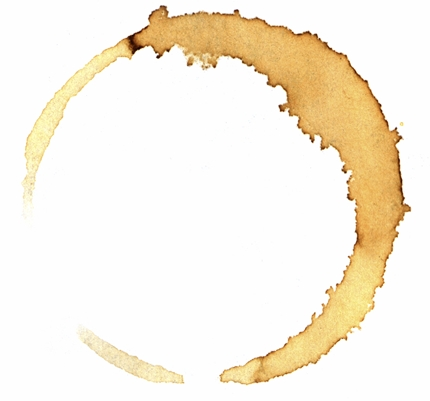
\includegraphics[width=4cm]{./images/cafe-mancha.jpg}
  \end{figure}
  \vspace{-10mm}
  \textbf{\tiny{Apoya tu cafe aqui}} \\
	\vspace{10mm}
  %%%%%%%%%%%%%%%%%%%%%%%%%%%%%%%%%%%%%%
  % Ingresa el mejor titulo que se te ocurra
  %%%%%%%%%%%%%%%%%%%%%%%%%%%%%%%%%%%%%%
	\textbf{\LARGE{Un modelo de simulación informático esta ayudando a encontrar respuestas para enfermedades como Alzheimer, el Parkinson o la enfermedad de Huntington. }}\\
	\vspace{4mm}
		\textbf{\large{Tomás Vera\\
  email: \href{mailto:vtomasv@gmail.com}{vtomasv@gmail.com}  } }\\
	\vspace{3mm}
	\textbf{\large{Universidad de Chile}}\\
	\textbf{\small{CC71T-1 Investigación en Cs. de la Computación.(Métodos,Técnicas,Persp.) }}\\
	\textbf{\large{Profesor: Claudio Gutierrez \\
  email: \href{mailto:cgutierr@dcc.uchile.cl}{cgutierr@dcc.uchile.cl}  } }\\
	\today
\end{center}

%%%%%%%%%%%%%%%%%%%%%%%%%%%%%%%%%%%%%%
% Resumen formal de la noticia
%%%%%%%%%%%%%%%%%%%%%%%%%%%%%%%%%%%%%%
\section*{\centering Resumen}
Las células están en constante movimiento, se dividen y se encargan de transportar moléculas en su interior. Un grupo de investigación de la Universidad del Sur de Dinamarca ha desarrollado modelo matemático\autocite{web:1} basado en ecuaciones diferenciales que permite simular lo que ocurre dentro de una célula viva y facilita la monitorización del tráfico intracelular.
De esta forma se pueden detectar fallos o perturbaciones en los procesos de transporte moleculares, el causante o factor implicado en ciertas enfermedades cuyas consecuencias pueden ser fatales. Es el caso del Alzheimer, el Parkinson o la enfermedad de Huntington, trastornos neurodegenerativos con muchas similitudes a nivel molecular.

En la actualidad existen varias técnicas de microscopía moderna para visualizar el tráfico intracelular. Es el caso de la Pérdida de Fluorescencia en el Foto-blanqueamiento (FLIP), que consiste en decolorar repetidamente una región específica de la célula mediante un pulso láser para observar la pérdida de fluorescencia en las partes no blanqueadas, donde se encuentran las moléculas de interés. Así se produce una reducción progresiva de movimiento del área blanqueada en la dirección de transporte.
El modelo creado por los investigadores permite realizar este analisis Pérdida de Fluorescencia en forma automática y realizar simulaciones para detectar mal funcionamiento en los transportes moleculares y así detectar enfermedades causadas por un mal funcionamiento de la proteína intracelular o del tráfico de la membrana.


%%%%%%%%%%%%%%%%%%%%%%%%%%%%%%%%%%%%%%
% Tu voz sobre el impacto de esta noticia
%%%%%%%%%%%%%%%%%%%%%%%%%%%%%%%%%%%%%%
\section{Opinion}
El avance del analisis de imágenes y de modelos de simulación esta permitiendo no solo realizar la simulación de tráfico intracelular sino que también esta llevando los modelos de detección de patrones a otro nivel. Si bien este es un ejemplo extraordinario de como las matematicas se unen con la informática para dar resultados a al medicina es increíble como hoy las distintas ciencias se complementan a fin de obtener resultados que aumentan el conocimiento.
Esta noticia para mi es el reflejo de que el trabajo en conjunto de todas las ciencias es el mejor paso a la hora de crear o romper las nuevas barreras del conocimiento.

%%%%%%%%%%%%%%%%%%%%%%%%%%%%%%%%%%%%%%
% Referencias sobre la noticia
%%%%%%%%%%%%%%%%%%%%%%%%%%%%%%%%%%%%%%
\section{Referencias\label{sec:references}}

\printbibliography[heading=none]


\section{Tu opinion es muy importante!}
\begin{figure}
    \centering
    
\includegraphics[width=4cm]{./images/vote.png}
    \captionsetup{justification=centering, singlelinecheck=false}
\end{figure}

\end{document}
